\documentclass[11pt,a4paper]{article}

\usepackage[a4paper,margin=23mm,headheight=15pt]{geometry}
\usepackage{fontspec}
\setmainfont{TeX Gyre Pagella}
\setsansfont{TeX Gyre Heros}
\setmonofont{DejaVu Sans Mono}[Scale=0.82]
\usepackage{microtype}
\usepackage{graphicx}
\usepackage{booktabs}
\usepackage{tabularx}
\usepackage{array}
\usepackage{amsmath}
\usepackage{siunitx}
\usepackage{xcolor}
\usepackage{listings}
\usepackage{caption}
\usepackage{float}
\usepackage{enumitem}
\usepackage{fancyhdr}
\usepackage{titlesec}
\usepackage[most]{tcolorbox}
\usepackage[colorlinks=true,linkcolor=blue!45!black,urlcolor=blue!55!black,citecolor=blue!45!black]{hyperref}

\newcommand{\StudentName}{Zhanyu Zhang}
\newcommand{\UoGID}{2959456}
\newcommand{\UESTCID}{2023300901013}
\newcommand{\ReportDate}{15 September 2026}


\definecolor{navy}{HTML}{173B57}
\definecolor{blue}{HTML}{2F6F9F}
\definecolor{orange}{HTML}{D66A1F}
\definecolor{ink}{HTML}{263238}
\definecolor{soft}{HTML}{F2F5F7}
\definecolor{codegreen}{HTML}{39754A}

\titleformat{\section}{\Large\bfseries\sffamily\color{navy}}{\thesection}{0.7em}{}
\titleformat{\subsection}{\large\bfseries\sffamily\color{blue}}{\thesubsection}{0.7em}{}
\titlespacing*{\section}{0pt}{2.2ex plus 0.5ex}{1.0ex}
\titlespacing*{\subsection}{0pt}{1.8ex plus 0.4ex}{0.7ex}

\pagestyle{fancy}
\fancyhf{}
\lhead{RTCSCA Lab 1}
\rhead{Registers, GPIO, Timers and Interrupts}
\cfoot{\thepage}
\renewcommand{\headrulewidth}{0.4pt}

\lstdefinestyle{cstyle}{
  language=C,
  basicstyle=\ttfamily\small,
  keywordstyle=\color{blue}\bfseries,
  commentstyle=\color{codegreen}\itshape,
  stringstyle=\color{orange},
  numbers=left,
  numberstyle=\tiny\color{gray},
  stepnumber=1,
  numbersep=8pt,
  frame=single,
  rulecolor=\color{black!15},
  backgroundcolor=\color{soft},
  breaklines=true,
  showstringspaces=false,
  tabsize=2,
  columns=fullflexible
}
\lstset{style=cstyle}

\newtcolorbox{resultbox}[1]{
  colback=blue!4,
  colframe=blue!65!black,
  boxrule=0.7pt,
  arc=1.5mm,
  title=\textbf{#1},
  coltitle=white,
  colbacktitle=blue!75!black
}

\begin{document}

\begin{titlepage}
  \centering
  \vspace*{18mm}
  {\sffamily\Large Real-Time Computer Systems and Computer Architecture\par}
  \vspace{16mm}
  {\sffamily\bfseries\fontsize{30}{36}\selectfont Laboratory 1\par}
  \vspace{4mm}
  {\sffamily\Large Registers, GPIO, Timers and Interrupts\par}
  \vspace{18mm}
  \begin{tcolorbox}[width=0.84\textwidth,colback=soft,colframe=blue!55!black,arc=2mm]
    \centering
    \begin{tabular}{@{}rl@{}}
      \textbf{Target device:} & STM32L073RZT6 \quad (Arm Cortex-M0+)\\
      \textbf{Board:} & NUCLEO-L073RZ\\
      \textbf{System clock:} & \SI{32}{\mega\hertz}\\
      \textbf{Toolchain:} & STM32CubeMX 6.17 / Keil MDK-ARM 5
    \end{tabular}
  \end{tcolorbox}
  \vfill
  \begin{tabular}{@{}>{\bfseries}rl@{}}
    Student: & \StudentName\\[2mm]
    Glasgow ID: & \GlasgowID\\[2mm]
    UESTC ID: & \UESTCID
  \end{tabular}
  \vfill
  {\large \today\par}
\end{titlepage}

\begin{abstract}
This laboratory implements direct GPIO register operations and interrupt-driven timing on an STM32 microcontroller. The register exercises establish how masks isolate and update individual fields. The firmware then reads the NUCLEO-L073RZ blue button through GPIOC, controls the built-in LD2 LED through GPIOA, and uses an external interrupt together with TIM2 to start and stop a \SI{1.5}{\second} blink sequence. The final Keil build completed with zero errors and zero warnings.
\end{abstract}

\tableofcontents
\clearpage

\section{Hardware and Project Configuration}

The implementation targets the STM32L073RZT6, which contains a \SI{32}{\mega\hertz} Arm Cortex-M0+ core, 192~KB ECC Flash, 20~KB RAM, and 6~KB ECC data EEPROM~\cite{stm32l073-ds}. The NUCLEO-L073RZ connects the green user LED LD2 to PA5 and the blue user button B1 to PC13~\cite{nucleo-um}.

\begin{table}[H]
\centering
\caption{Lab 1 peripheral configuration.}
\begin{tabularx}{0.92\textwidth}{@{}l l X@{}}
\toprule
\textbf{Resource} & \textbf{Setting} & \textbf{Purpose}\\
\midrule
PA5 & GPIO push-pull output & Drives the active-high LD2 LED\\
PC13 & Falling-edge EXTI input & Detects a press of the B1 button\\
TIM2 & Internal clock, update interrupt & Generates the LED toggle interval\\
SYSCLK & HSI16, PLL $\times 4 / 2$ & Supplies a \SI{32}{\mega\hertz} system and timer clock\\
\bottomrule
\end{tabularx}
\end{table}

STM32CubeMX generates the clock, GPIO, TIM2, and NVIC initialization. Independently written application code is separated into the project-local \texttt{Lab1/Inc} and \texttt{Lab1/Src} directories.

\section{Task 1: GPIOB Pin 5 Register Configuration}

The task uses the four-bit \texttt{GPIOx\_CRL} pin field described by the STM32F1 register model in the laboratory brief~\cite{rm0008}. Pin 5 occupies bits 23:20. General-purpose push-pull output mode requires \texttt{CNF[1:0] = 00}, and the \SI{50}{\mega\hertz} output selection requires \texttt{MODE[1:0] = 11}; therefore the complete nibble is \texttt{0011}.

\subsection{Step-by-step bitwise operations}

Let the untouched register bits be written as \texttt{x}. The field mask is

\[
M = 0xF \ll 20 = \mathtt{0x00F00000}.
\]

The starting register is represented symbolically as

\[
\mathtt{xxxxxxxx\ xxxxxxxx\ xxxxxxxx\ xxxxxxxx}.
\]

First, clear bits 23:20:

\begin{lstlisting}
GPIOB->CRL &= ~0x00F00000U;
\end{lstlisting}

The result is

\[
\mathtt{xxxxxxxx\ 0000xxxx\ xxxxxxxx\ xxxxxxxx}.
\]

Second, place \texttt{0011} in the field:

\begin{lstlisting}
GPIOB->CRL |= 0x00300000U;
\end{lstlisting}

The result is

\[
\mathtt{xxxxxxxx\ 0011xxxx\ xxxxxxxx\ xxxxxxxx}.
\]

Figure~\ref{fig:task1-field} shows that only the PB5 field changes.

\begin{figure}[H]
  \centering
  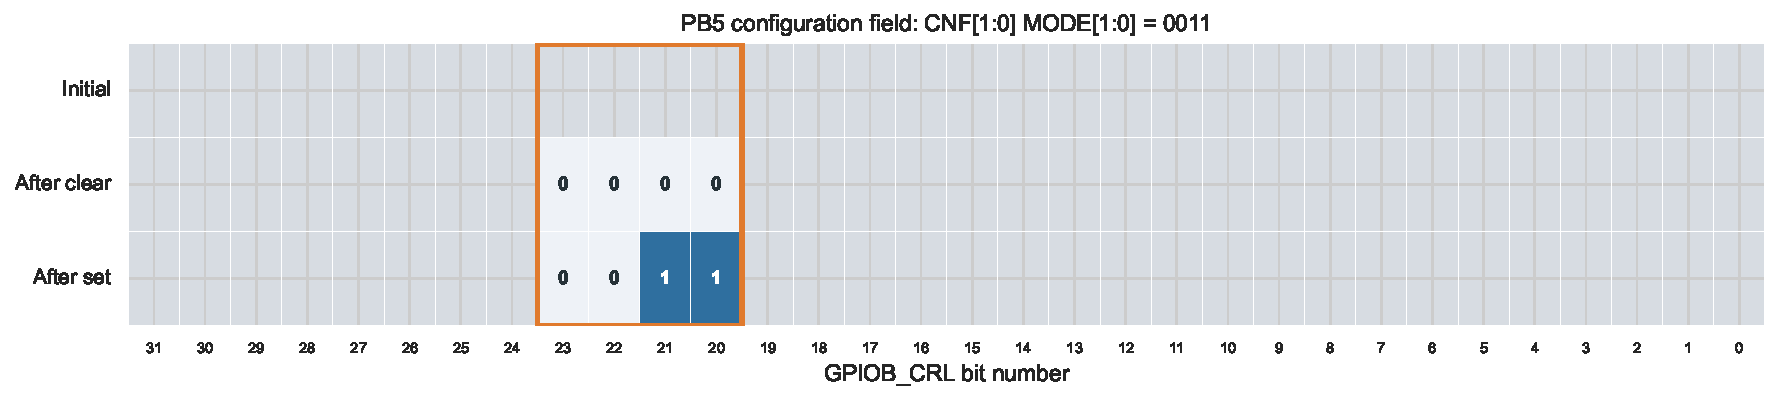
\includegraphics[width=\textwidth]{figures/task1_register_field.pdf}
  \caption{Bit-field progression for GPIOB pin 5. Grey cells are preserved bits.}
  \label{fig:task1-field}
\end{figure}

\subsection{Minimum-step code}

The clear and set transformations can be combined into one read-modify-write statement:

\begin{lstlisting}
GPIOB->CRL = (GPIOB->CRL & ~(0xFU << 20U)) | (0x3U << 20U);
\end{lstlisting}

The mask preserves all fields other than PB5, while the encoded value writes \texttt{0011} into bits 23:20. In the STM32L073 firmware project, the equivalent output function is generated through the STM32L0 \texttt{MODER}, \texttt{OTYPER}, and \texttt{OSPEEDR} register model~\cite{rm0367}.

\section{Task 2: Evaluating a GPIO Input Bit}

The expression is

\begin{lstlisting}
bool Pinx = (GPIOx->IDR & (1U << GPIOx_PIN_N)) != 0U;
\end{lstlisting}

It evaluates in three operations:

\begin{enumerate}[leftmargin=2em]
  \item \texttt{1U << GPIOx\_PIN\_N} creates a mask with a single one at the selected pin position.
  \item Bitwise AND removes every other input bit and retains only the selected pin state.
  \item Comparison with zero converts the masked value to \texttt{false} or \texttt{true}.
\end{enumerate}

For pin 13, the mask is $1 \ll 13 = \mathtt{0x2000}$. If \texttt{GPIOC->IDR} is \texttt{0x2400}, then

\[
\mathtt{0x2400 \ \& \ 0x2000 = 0x2000},
\]

which is non-zero, so \texttt{Pinx} is \texttt{true}. If the register value is \texttt{0x0400}, the AND result is zero and \texttt{Pinx} is \texttt{false}. The \texttt{bool} type is supplied by \texttt{<stdbool.h>}.

\section{Task 3: Button-Controlled LED with IDR and ODR}

B1 is read from bit 13 of \texttt{GPIOC->IDR}. A press produces the active input level used by the falling-edge board configuration. PA5 is then set or cleared in \texttt{GPIOA->ODR}; the other output bits remain unchanged.

\lstinputlisting[caption={Task 3 register-level implementation.},label={lst:task3}]{../Firmware/Lab1/Lab1/Src/task3_polling.c}

The Boolean expression normalizes the button state, after which the two ODR operations directly implement the required LED-on and LED-off behavior.

\section{Task 4: Interrupt-Driven 1.5 s Blinking}

\subsection{Timer calculation}

TIM2 receives a \SI{32}{\mega\hertz} clock because APB1 uses a divider of one. A \SI{1}{\kilo\hertz} counter tick is formed with a division factor of 32,000:

\[
f_{\mathrm{counter}} = \frac{32\,000\,000}{31999 + 1} = \SI{1000}{\hertz}.
\]

Counting 1,500 ticks produces the requested interval:

\[
T_{\mathrm{update}} = \frac{1499 + 1}{1000} = \SI{1.5}{\second}.
\]

\begin{resultbox}{TIM2 values}
\begin{center}
\begin{tabular}{@{}ll@{}}
Timer & \texttt{TIM2}\\
Prescaler register & \texttt{31999}\\
Counter period register & \texttt{1499}\\
Counter mode & Up\\
Update interrupt & Enabled\\
\end{tabular}
\end{center}
\end{resultbox}

The generated initialization applies these values:

\begin{lstlisting}
htim2.Instance = TIM2;
htim2.Init.Prescaler = 31999;
htim2.Init.CounterMode = TIM_COUNTERMODE_UP;
htim2.Init.Period = 1499;
htim2.Init.ClockDivision = TIM_CLOCKDIVISION_DIV1;
htim2.Init.AutoReloadPreload = TIM_AUTORELOAD_PRELOAD_DISABLE;
HAL_TIM_Base_Init(&htim2);
\end{lstlisting}

\subsection{External and internal interrupt behavior}

The PC13 falling edge calls \texttt{HAL\_GPIO\_EXTI\_Callback}. The first accepted press turns LD2 on, resets TIM2, and starts update interrupts. Each TIM2 period callback toggles PA5. The next accepted press stops TIM2 with \texttt{HAL\_TIM\_Base\_Stop\_IT} and clears PA5. A \SI{30}{\milli\second} time gate suppresses the extra edges produced by the mechanical button.

\begin{figure}[H]
  \centering
  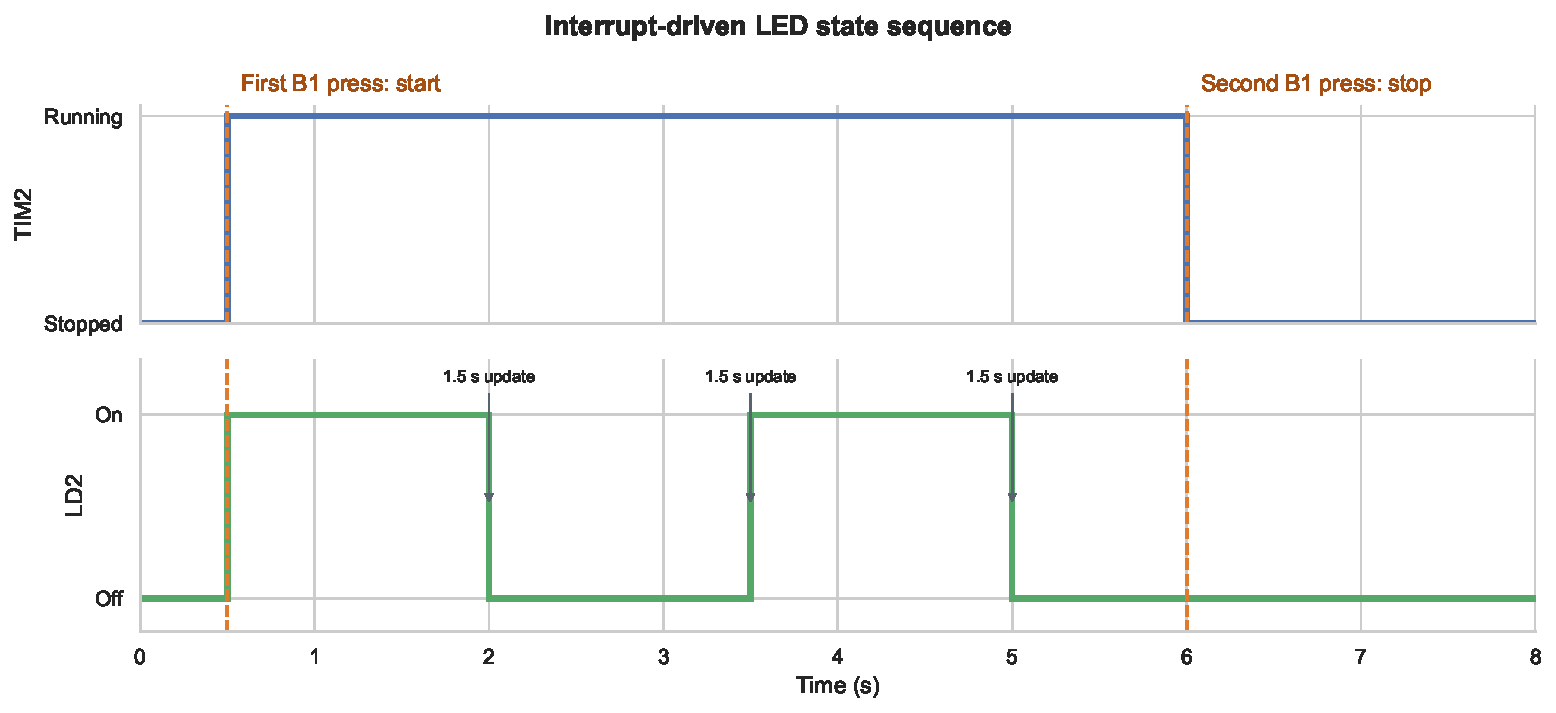
\includegraphics[width=0.98\textwidth]{figures/task4_timing.pdf}
  \caption{Example Task 4 state sequence. Timer updates toggle LD2 every \SI{1.5}{\second}.}
  \label{fig:task4-timing}
\end{figure}

\lstinputlisting[caption={Task 4 application module.},label={lst:task4}]{../Firmware/Lab1/Lab1/Src/lab1_app.c}

The main loop executes \texttt{\_\_WFI()} and contains no delay call. All LED timing is generated by the timer update interrupt, while the button transition is captured by EXTI.

\section{Build Results}

The STM32CubeMX-generated Keil project was compiled with Arm Compiler 5.06 update 7. Table~\ref{tab:build} summarizes the resulting image.

\begin{table}[H]
\centering
\caption{Keil build summary.}
\label{tab:build}
\begin{tabular}{@{}lr@{}}
\toprule
\textbf{Item} & \textbf{Result}\\
\midrule
Errors & 0\\
Warnings & 0\\
Code & 4,876 bytes\\
Read-only data & 252 bytes\\
Read-write data & 28 bytes\\
Zero-initialized data & 1,700 bytes\\
\bottomrule
\end{tabular}
\end{table}

The register masks preserve unrelated GPIO pins, and the timer equation matches the generated prescaler and auto-reload values. The interrupt state sequence satisfies the two button actions: start the timed blink and stop with the LED off.

\section{Conclusion}

Together, the four tasks connect register fields with event-driven firmware. Masking and shifting provide deterministic GPIO configuration and sampling, while EXTI and TIM2 separate asynchronous user input from periodic LED timing. The resulting project uses the STM32L073RZT6 at \SI{32}{\mega\hertz}, implements the \SI{1.5}{\second} interval without a delay function, and compiles cleanly in Keil MDK-ARM.

\begin{thebibliography}{9}
\bibitem{labbrief}
RTCSCA, \emph{Lab 1: Registers, Timers and Interrupts}, 2026--2027.

\bibitem{stm32l073-ds}
STMicroelectronics, \emph{STM32L073xx Datasheet}, DS10685.\\
\url{https://www.st.com/resource/en/datasheet/stm32l073rz.pdf}

\bibitem{rm0367}
STMicroelectronics, \emph{STM32L0x3 Reference Manual}, RM0367.\\
\url{https://www.st.com/resource/en/reference_manual/dm00095744.pdf}

\bibitem{nucleo-um}
STMicroelectronics, \emph{STM32 Nucleo-64 Boards User Manual}, UM1724.\\
\url{https://www.st.com/resource/en/user_manual/dm00105823.pdf}

\bibitem{rm0008}
STMicroelectronics, \emph{STM32F1 Reference Manual}, RM0008.\\
\url{https://www.st.com/resource/en/reference_manual/cd00171190.pdf}
\end{thebibliography}

\end{document}
